% Fichier généré automatiquement par tools/generate_corrections.py.
% Source : STAT/STAT-03-Demarche/06_TR/06_TR.tex
% Statut : complété (4/4 question(s)).
\begin{corrigebox}[Corrigé complété]
\CorrigeQuestion{1}
\CorrigeSource{Réponse reprise d'un exercice homonyme de la banque ; la provenance exacte est indiquée dans le commentaire du fichier.}
% Réponse reprise de : DYN/DYN-05-Methode/06_TR/06_TR.tex
\par\medskip\begin{center}\captionsetup{type=figure}
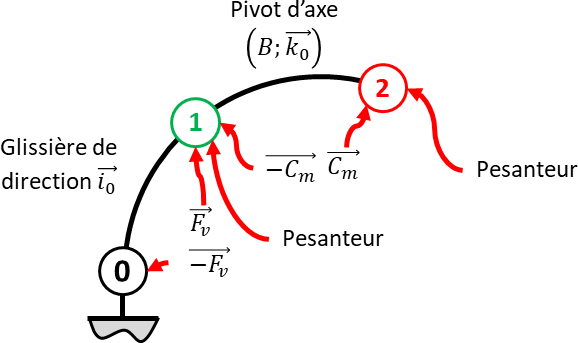
\includegraphics[width=.7\linewidth]{../../../DYN/DYN-05-Methode/06_TR/images/06_TR_02_Cor}
\end{center}\par\medskip
\CorrigeQuestion{2}
On écrit le torseur dans un point de réduction adapté. La résultante
        est obtenue par la définition correspondante et le moment est transporté par
        $\vec M_A=\vec M_B+\overrightarrow{AB}\wedge\vec R$. Les composantes sont ensuite
        projetées dans la base demandée.
\CorrigeQuestion{3}
On écrit le torseur dans un point de réduction adapté. La résultante
        est obtenue par la définition correspondante et le moment est transporté par
        $\vec M_A=\vec M_B+\overrightarrow{AB}\wedge\vec R$. Les composantes sont ensuite
        projetées dans la base demandée.
\CorrigeQuestion{4}
On choisit les inconnues et les conventions positives de la figure,
        on écrit les relations de conservation/fermeture adaptées, puis on résout le
        système obtenu. Le résultat symbolique doit être homogène et vérifié dans les cas
        limites (entrée nulle, rapport unitaire ou position de référence).
\end{corrigebox}
